\section{Theorie}
\label{sec:Theorie}

Der Franck-Hertz-Versuch belegt die Aussage von Niels Bohrs Atommodell, dass Atome diskrete
Energieniveaus besitzen.
Dies bedeutet, dass Atome -- in diesem Fall Quecksilber -- durch diskrete Anregungsenergien
in einen höherenergetischen Zustand versetzt werden können und bei der Rückkehr in den
Anfangszustand einen Lichtquanten mit einer Energie emittieren, die der Energiedifferenz zwischen
Anfangszustand und angeregtem Zustand, also
\begin{equation}
	\label{eqn:photonemission}
	\symup{h} \nu = E_1 - E_0
\end{equation}
entspricht. Hierbei entspricht $\symup{h}$ dem Planck'schen Wirkungsquantum und $\nu$ der
Frequenz des emittierten Lichtquants.
Die Anregung der Atome kann durch zwei unterschiedliche Methoden realisiert werden.
Zum Einen durch Wechselwirkung elektromagnetischer Strahlung mit den Atomen.
Zum Anderen mit den hier betrachteten Stoßprozessen von Elektronen mit den Atomen, den
sogenannten \textbf{Elektronenstoßexperimenten}.
Um dieses Phänomen näher zu behandeln wird zunächst der prinzipielle Aufbau des
Franck-Hertz-Versuchs erläutert.
\subsection{Prinzipieller Aufbau des Franck-Hertz-Versuchs}
\begin{figure}
  \centering
  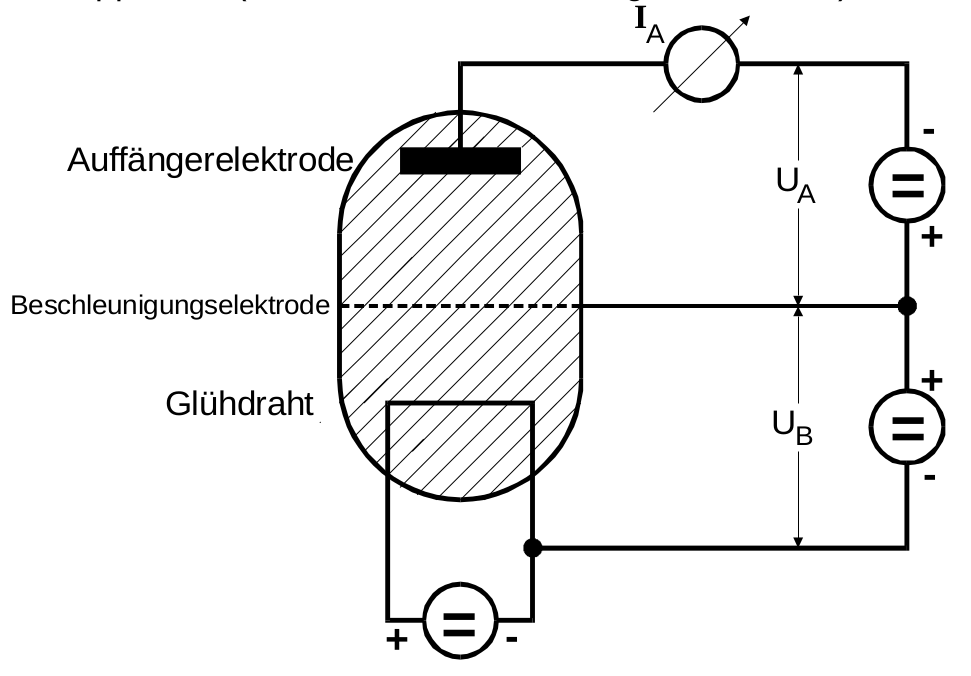
\includegraphics[width=0.7\textwidth]{Bilder/aufbau.png}
  \caption{Prinzipieller Aufbau des Frack-Hertz-Versuchs \cite{Anleitung}.}
  \label{fig:franckhertztheory}
\end{figure}
Der prinzipielle Aufbau des Franck-Hertz-Versuchs ist in Abbildung \ref{fig:franckhertztheory}
dargestellt.
In einem evakuierten Gefäß befinden sich ein Glühdraht, eine Beschleunigungselektrode, eine
Auffängerelektrode und die Quecksilberatome.
Die Dichte der Quecksilberatome ist gemäß der Dampfdruck-Kurve temperaturabhängig.
Der Glühdraht, bestehend aus einem Material mit niedriger Austrittsarbeit, wird durch eine
Gleichspannung erhitzt und es treten gemäß dem glühelektrischen Effekt Elektronen
aus dem Draht aus.
Da zwischen dem Glühdraht und der Beschleunigungselektrode eine positive Spannung anliegt,
erhalten die Elektronen -- vorrausgesetzt sie besitzen unmittelbar nach dem Austritt aus dem
Draht keine kinetische Energie -- bis zur Beschleunigungselektrode die kinetische Energie
\begin{equation}
	E_{\mathrm{kin}} = \frac{\symup{m}_0 v_{\mathrm{vor}}^2}{2} = \symup{e}_0 U_{\mathrm{B}} \mathrm{,}
\end{equation}
wobei $\symup{m}_0$ der Elektronenmasse und $\symup{e}_0$ der Elementarladung entspricht.
Am Ende des Gefäßes ist eine Auffängerelektrode angebracht, die ein Gegenfeld mit der Spannung
$U_{\mathrm{A}}$ erzeugt, sodass nur Elektronen die Auffängerdiode erreichen, die die
Ungleichung
\begin{equation}
	\frac{\symup{m}_0}{2} v_{\mathrm{z}}^2 \geq \symup{e}_0 U_{\mathrm{A}}
\end{equation}
erfüllen. Das $v_{\mathrm{z}}$ stellt die z-Komponente des Geschwindigkeitsvektors dar,
angenommen die z-Achse liegt in Richtung der Auffängerelektrode.

Treffen die Elektronen auf Quecksilberatome können zwei Arten von Stößen auftreten: die
Elastischen und die Unelastischen. Bei den elastischen Stößen reicht die Energie der Elektronen
nicht aus um das Atom anzuregen. Aufgrund der großen Massendifferenz der beiden Stoßpartner
kann die Energieabgabe der Elektronen vernachlässigt werden. Allerdings erfahren die Elektronen
beim elastischen Stoß eine Richtungsänderung.
Bei den unelastischen Stößen hingegen besitzen die Elektronen eine hinreichend große
Energie um das Atom in einen höherenergetischen Zustand zu versetzen und übertragen diesen
dafür nötigen Energiebetrag $E_1-E_0$ auf das Atom.
Das angeregte Atom relaxiert in den Anfangszustand und emittiert dabei ein Photon gemäß
Formel \eqref{eqn:photonemission}.
\begin{figure}
  \centering
  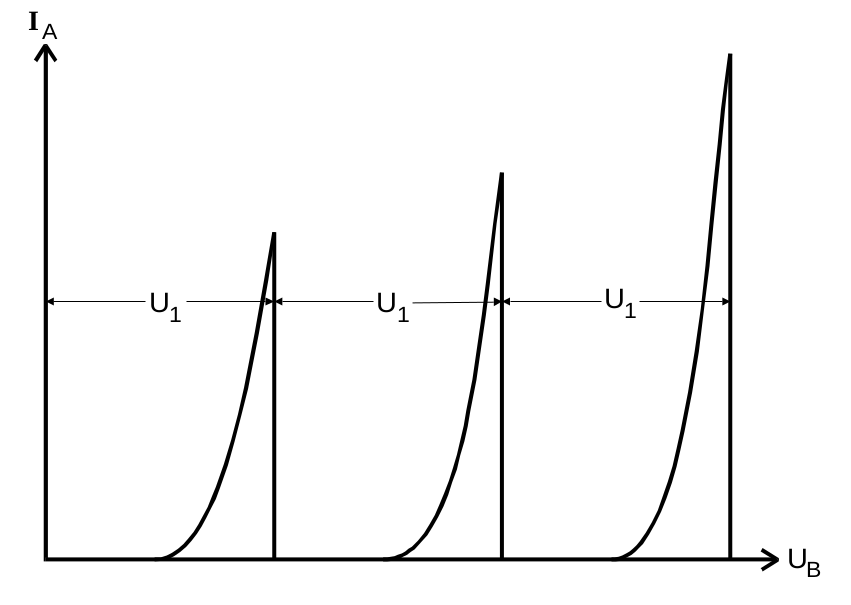
\includegraphics[width=0.7\textwidth]{Bilder/ideale_hertzkurve.png}
  \caption{Charakteristische Gestalt der idealen Franck-Hertz-Kurve \cite{Anleitung}.}
  \label{fig:franckhertzkurve}
\end{figure}
Durch diese Stoßprozesse ergibt sich ein theoretischer Verlauf des an der Auffängerelektrode
gemessenen Auffängerstroms $I_{\mathrm{A}}$ in Abhängigkeit von der Beschleunigungsspannung
$U_{\mathrm{B}}$ wie in Abbildung \ref{fig:franckhertzkurve} zu sehen ist.
Dieser Graph wird als \textbf{Franck-Hertz-Kurve} bezeichnet.
Es wird idealisierend von einer monoenergetischen Energieverteilung der Elektronen ausgegangen.
Dann werden die Elektronen beschleunigt, bis sie eine hinreichend hohe Energie besitzen, um
das Gegenfeld zu durchqueren. Die Anzahl der Elektronen steigt mit steigender
Beschleunigungsspannung bis ein instantaner Abfall des Auffängerstroms erfolgt. Die Elektronen
haben an diesem Punkt genau die Energie, um die Quecksilberatome anzuregen. Dieser Vorgang
wiederholt sich periodisch.
Außerdem lässt sich an der Franck-Hertz-Kurve das Anregungspotential als äquidistanter
Abstand der Maxima zu
\begin{equation}
	U_1 = \frac{E_1-E_0}{\symup{e}_0}
\end{equation}
bestimmen.
Im Folgenden werden Einflüsse diskutiert, die zur Folge haben, dass die Franck-Hertz-Kurve nicht
wie in Abbildung \ref{fig:franckhertzkurve} bestimmt werden kann.
\subsection{Einflüsse auf die Gestalt der Franck-Hertz-Kurve}
\subsubsection{Einfluss des Kontaktpotentials}
\begin{figure}
  \centering
  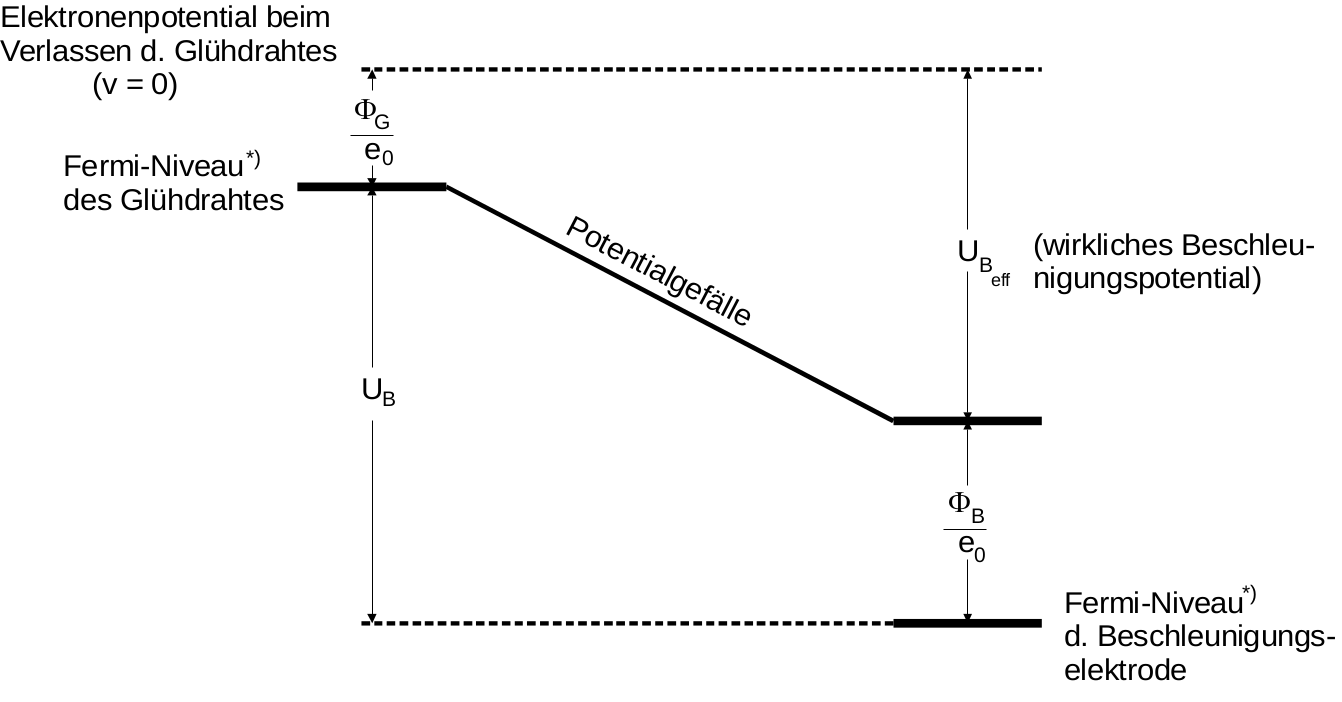
\includegraphics[width=\textwidth]{Bilder/fermi_niveau.png}
  \caption{Darstellung der Potentialverhältnisse zwischen Glühkathode und Beschleunigungselektrode \cite{Anleitung}.}
  \label{fig:potentialverh}
\end{figure}
In der Regel besteht der Glühdraht aus einem Material mit niedriger Austrittsarbeit
$\Phi_{\mathrm{G}}$, einer niedrigeren als bei der Beschleunigungselektrode $\Phi_{\mathrm{B}}$.
Dadurch verändert sich die effektive Beschleunigungsspannung $U_{\mathrm{B,eff}}$ wie in
Abbildung \ref{fig:potentialverh} illustriert.
Es ergibt sich das effektive Beschleunigungspotential
\begin{equation}
	U_{\mathrm{B,eff}} = U_{\mathrm{B}} - \frac{\Phi_{\mathrm{B}}-\Phi_{\mathrm{G}}}{\symup{e}_0} \mathrm{.}
\end{equation}
Hierbei wird der Subtrahend
\begin{equation}
	K:=\frac{\Phi_{\mathrm{B}}-\Phi_{\mathrm{G}}}{\symup{e}_0}
\end{equation}
als \textbf{Kontaktpotential} bezeichnet.
Die Franck-Hertz-Kurve wird durch diesen Einfluss um das Kontaktpotential $K$ verschoben.
\subsubsection{Einfluss des Energiespektrums der Elektronen}
Ein weiterer Einfluss auf die Franck-Hertz-Kurve ist die nicht gegebene monoenergetische
Energieverteilung der Elektronen. Die Elektronen besitzen nach der Fermi-Dirac-Statistik ein
statistisch verteiltes Energiespektrum im Draht und es ergibt sich somit nach Austritt der
Elektronen aus dem Draht eine Geschwindigkeitsverteilung. Dies hat zur Folge, dass die Maxima
der Franck-Hertz-Kurve nicht mehr einer bestimmten Beschleunigungsspannung zuzuordnen sind,
sondern sich aufgrund der statistischen Verteilung über ein Intervall erstrecken.
\subsubsection{Einfluss des Dampfdruckes}
Voraussetzung für den Franck-Hertz-Versuch sind Stöße der Elektronen mit Atomen.
Daher muss die mittlere freie Weglänge $\bar{w}$ klein gegen den Abstand $a$ zwischen Kathode
und Beschleunigungselektrode sein.
Die mittlere freie Weglänge ergibt sich über Sättigungsdampfdruck $p$ gemäß der kinetischen
Gastheorie zu
\begin{equation}
	\label{eqn:freiewegl}
	\bar{w} = \frac{0.0029}{p_{\mathrm{sätt}}} \mathrm{.}
\end{equation}
\begin{figure}
  \centering
  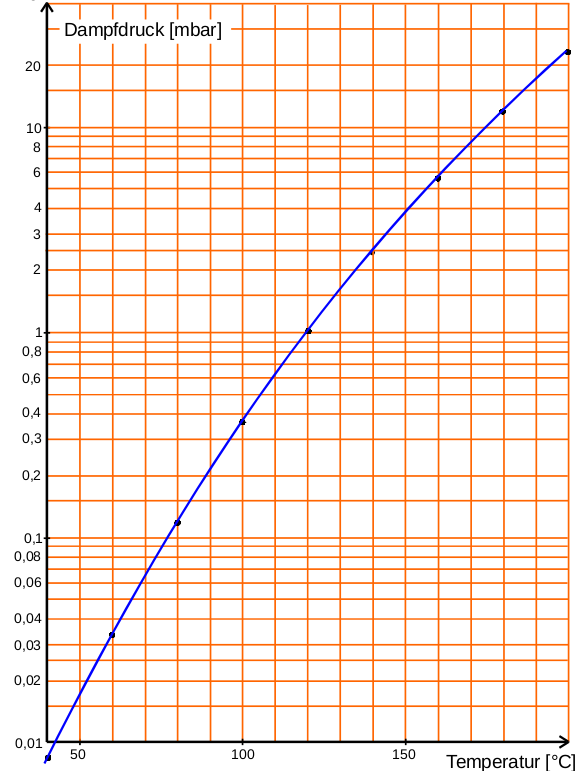
\includegraphics[width=0.7\textwidth]{Bilder/dampfdruckkurve.png}
  \caption{Dampfdruckkurve des Quecksilbers \cite{Anleitung}.}
  \label{fig:dampfi}
\end{figure}
